%\documentclass{mai_book}
%\defaultfontfeatures{Mapping=tex-text}
%\setmainfont{DejaVuSerif}
%\setdefaultlanguage{russian}
%\usepackage{amsmath}
%\usepackage{floatflt}
%\usepackage{wrapfig,lipsum,booktabs}
%\begin{document}
\textbf{2.}  Для $d > 0$ (вещественное квадратичное расширение) ситуация\linebreak
более сложная. Существуют, как в мнимом случае, значения $d$, для ко- \linebreak торых соответствующее кольцо есть КГИ, и другие значения, для ко-\linebreak торых оно таковым не является. Таблицы, предоставляющие этот вид\linebreak
информации (для $d$, относящегося или нет к определенному типу), су-\linebreak ществуют в литературе, например, [28]. Там также утверждается, что\linebreak
самое маленькое $d > 0$, для которого соответствующее кольцо не явля-\linebreak ется КГИ, есть $d = 10.$ В настоящий момент неизвестно, существует\linebreak
ли бесконечное множество таких положительных $d$, что кольцо целых\linebreak
чисел в $Q[\sqrt{d}]$ является КГИ.
\ \newline
\hspace*{10pt} \textbf{Евклидовость} квадратичных вещественных колец ставит также\linebreak
другие открытые проблемы. Известно, например, что кольца, являющиеся\linebreak евклидовыми для \textit{абсолютной нормы} $|N|$, исчерпываются кольцами,\linebreak
соответствующими шестнадцати значениям $d$ (сравнить [80] или [159]):
$$d = 2,\hspace*{10pt} 3,\hspace*{10pt} 5,\hspace*{10pt} 6,\hspace*{10pt} 7,\hspace*{10pt} 11,\hspace*{10pt} 13,\hspace*{10pt} 17,\hspace*{10pt} 19,\hspace*{10pt}$$
	$$\hspace*{95pt}21,\hspace*{10pt} 29,\hspace*{10pt} 33,\hspace*{10pt} 37,\hspace*{10pt} 41,\hspace*{10pt} 57,\hspace*{10pt} 73.$$
В статье Уайнбергера [175] доказано, что из \textbf{ослабленной гипотезы\linebreak
Римана} следует, что всякое вещественное квадратичное кольцо\linebreak евклидово коль скоро оно есть \textbf{КГИ}. Однако неизвестно, можно ли в явном\linebreak
виде указать вещественное евклидово квадратичное кольцо, не \linebreak фигурирующее в данном месте. Например, квадратичное кольцо, \linebreak соответствующее $d$ = 14, является КГИ и, согласно сделанному выше примечанию, возможно, евклидово. Однако этот тезис на настоящий момент
мы не можем ни доказать, ни опровергнуть. В самом деле, результат\linebreak
Уайнбергера утверждает, что при условии справедливости ослабленной\linebreak гипотезы Римана, всякое кольцо целых чисел (неважно какого\linebreak поля), за исключением 4 мнимых квадратичных колец, соответствующих\linebreak
$d$ = —163, —67, —43, —19, является евклидовым, \textbf{как только оно явля-\linebreak
ется КГИ}.\newline
\hspace*{10pt} В связи с этим некоторые математики ввели понятия квазиевклидовых колец (см. статью Кука [54] или диссертацию Буажо [31]). Эти\linebreak
авторы выражают в явном виде квазиевклидовы деления в неко-\linebreak торых вещественных квадратичных кольцах, достаточные для вычисле-\linebreak ния НОД. Вот некоторые значения $d$, для которых соответствующее
кольцо является квазиевклидовым (значения $d$, для которых соотве-\linebreak тствующее кольцо является евклидовым по отношению к абсолютному\linebreak
значению нормы, были исключены);
$$d = 14,22,23,31,38,43,46,47,53,61,69,$$
$$\hspace*{100pt}77,89,93,97,113,129,133,137,181,253.$$\linebreak\pagebreak

% 254 страница

\noindent Для этих значений $d$, кажется, ничего не известно о евклидовости со-\linebreak ответствующих колец.\\
\hspace*{10pt}Кроме того, Васерштейн в [171] доказал, что \textbf{вещественное} квадратичное кольцо будет квазиевклидовым, если оно есть \textbf{КГИ}. Следовательно, ситуация вполне предсказуема и мотивирует введение класса\linebreak
квазиевклидовых колец. В самом деле, последний результат наиболее\linebreak
общий. Он утверждает, что всякое \textbf{КГИ} целых чисел неважно какого\linebreak
числового поля, исключая 4 упомянутых выше квадратичных кольца\linebreak
(с $d$ = —163, —67, —43, —19), является квазиевклидовым.
\\
 \newline
\noindent\textbf{21. Нахождение колец мнимых квадратичностей}\\
 \newline
\hspace*{10pt}Пусть А — кольцо целых чисел мнимого квадратичного расширения\linebreak
$Q(\sqrt{d})$ поля рациональных чисел, где $d$ < 0 — целое число и $|d|$ не имеет\linebreak
нетривиальных квадратных множителей.\\
 \newline
 \hspace*{10pt}\textbf{a.} Определить группу единиц кольца $A$.\\
 \newline
  \hspace*{10pt}\textbf{b.} Пусть $B$ — евклидово кольцо, не являющееся полем, и\linebreak
$\varphi : B$ $\rightarrow$ $\mathbb {N}$ — евклидов алгоритм. Предположим, что все единицы в\linebreak
$B$ исчерпываются ±1. Рассматривая $\varphi$-минимальный элемент, доказать\linebreak
наличие $b \in B$ такого, что $B/(b)$ поле $\mathbb{Z}_2$ или $\mathbb {Z}_3$.
\\
 \newline
  \hspace*{10pt}\textbf{c.} Используя упражнение 20 и то, что число элементов кольца  $A/(z)$\linebreak
есть норма в $\mathbb {Z}$ (см. упражнение 12), доказать, что $A$ — евклидово тогда\linebreak
и только тогда, когда $d \in$  \{ —11, —7, —3, —2, —1\}. 
\\
 \newline
\noindent\textbf{22. Вычисление НОД с помощью двоичных операций}\\
 \newline
\hspace*{10pt} На машине, располагающей только следующими арифметическими\linebreak
операциями над целыми числами — сложение, вычитание, деление и\linebreak
умножение на степень двойки, а также критерием четности, необходимо\linebreak написать алгоритм вычисления НОД двух целых чисел.
 \newline
\hspace*{10pt} Если $а = 2^\alpha a'$ и $b = 2^\beta b'$, то какое соотношение связывает НОД$(a, b)$\linebreak
и НОД$(a', b')$? Отсюда просто вывести алгоритм вычисления НОД на\linebreak
рассматриваемой машине. Примените этот алгоритм к 1610 и 1000.\linebreak Какой вывод можно сделать с точки зрения эффективности?\\
\hspace*{10pt} Можно \textit{объединить} этот алгоритм с алгоритмом Евклида, используя\linebreak деление четного остатка: $a = bq + r$ c $|r| < |b|$ и четным $r$. Записать\linebreak
и поэкспериментируйте с программой вычисления НОД, основанной на\linebreak
этом делении.\pagebreak

% 255 страница

\noindent\textbf{23. Другое соотношение для последовательности Фибоначчи}\\\\
\hspace*{10pt}Пусть $F_n$ обозначает $n$-ое число Фибоначчи. Доказать, что $F_{n +m}$ =\linebreak
$F_m F_{n+1}+F_{m-1}F_n$ (доказано в упражнении 13 главы I). Вывести отсюда,\linebreak
что НОД($F_n, F_m$ ) = $F_{\text{НОД}(n, m)}$ (результат, принадлежащий Лукасу).\\\\
\noindent\textbf{24. Вычисление НОД $n$-ки целых чисел}\\
\\
\noindent\hspace*{10pt} Начиная с соотношения, полученного в начале раздела 6.3:\linebreak
НОД(0,0 . . . 0, $a$, 0 . . . 0, 0) = $a$ и, если $u_1\neq 0$, то НОД($u_1$, . . . ,$u_n$ ) =\linebreak
НОД($u_1$,$u_2$ mod $u_1$, . . . ,$u_n$ mod $u_1$) и, используя операцию \textit{Rotate\_Left}, \linebreak
определенную соотношением \textit{Rotate\_Left} (($u_1$, $u_2$, . . . ,$u_n$)) = ($u_2$, . . . ,\linebreak
$u_n$, $u_1$), можно написать алгоритм вычисления НОД $n$-ок целых чисел\linebreak
глобальным образом:
% Программа на СИ

\begin{lstlisting}[mathescape=true]
while(1){ 
 Number_of_zeros = 0; 
 for(int i = 0; i < n; i++){ 
  Rotate_left(u); 
  if(u[1] != 0) break; 
  Number_of_zeros = Number_of_zeros + 1;} 
 if(Number_of_zeros >= n - 1) break; 
 for(int i = 2; i < n; i++){ 
  u[i] = u[i]%u[1];}}
\end{lstlisting}
 \hspace*{10pt}\textbf{a.} Доказать, что если число нулей в массиве $u$ меньше или равно \linebreak
  $n$ $-$ 2, то в каждой итерации, кроме, быть может, первой, одна из\linebreak
компонент $u$ строго уменьшается. Вывести отсюда, что этот алгоритм\linebreak
эффективным образом вычисляет НОД чисел $u_i$.\\\\
 \hspace*{10pt}\textbf{b.} Перетасовка массива — не очень эффективная операция в программе.\linebreak
 Построить алгоритм вычисления НОД и целых чисел, аналогичный\linebreak предыдущему, но использующий подвижный указатель в \linebreak массиве вместо его сдвига.\\\\
  \hspace*{10pt}\textbf{c.} Можно легко построить еще более эффективный алгоритм,\linebreak
   используя два указателя в массиве вместо одного, и рассмотреть только\linebreak
часть массива, содержащегося между этими двумя индексами.\\
\\
\noindent\textbf{25. Странный алгоритм Евклида}\\\\
\hspace*{10pt} 
Доказать, что отображение $\varphi : \mathbb{Z}$ $\rightarrow$ $\mathbb {N}$, определенное через $\varphi(n) = |n|$\linebreak
при $n \neq 5$  и $\varphi(5) = 100$, является алгоритмом Евклида на $\mathbb{Z}$.\pagebreak

%256 страница

\noindent\textbf{26. Возрастающие алгоритмы Евклида}\\
\hspace*{10pt} Пусть $\varphi$ — алгоритм Евклида на кольце $A$. Определим $\bar{ \varphi}$  cследующим\linebreak
образом: $\bar{ \varphi}$(0) = $\varphi$(0) и, если $a\neq0$, то $\bar{ \varphi}(a)$=min$\{ \varphi(b)$ | $b \in Aa \backslash \{0\} \}.$\\\\
\hspace*{10pt}\textbf{a.} Доказать, что $\bar{ \varphi}$ — алгоритм Евклида, мажорируемый  $\varphi$.
\\
\hspace*{10pt}\textbf{b.} Доказать, что для ненулевых $a$ и $b$ $\bar{ \varphi}$ удовлетворяет соотношению:\linebreak
$a$ | $b$ $\Rightarrow \bar{ \varphi}(a) \leq \bar{ \varphi}(b).$\\
\hspace*{10pt}\textbf{c.} При тех же предположениях доказать, что если $a$ | $b$ и \linebreak $\bar{ \varphi}(a) = \bar{ \varphi}(b)$, то $Aa=Ab$.\\
\\
\noindent\textbf{27. Самый малый алгоритм Евклида на $\mathbb{Z}$}\\\\
\hspace*{10pt} Доказать, что отображение $\varphi$, ставящее каждому целому числу $b \in\mathbb{Z}$ \linebreak
в соответствие количество двоичных цифр в двоичной записи $|b|$,\linebreak
является алгоритмом Евклида на $\mathbb{Z}$ и что этот алгоритм самый малый\linebreak
алгоритм Евклида на $\mathbb{Z}$ (эта ограниченность, удобства ради, рассма-\linebreak
тривается на алгоритмах со значениями в $\mathbb{N}$).
\\
\\
\noindent\textbf{28. Реализация кольца целых чисел Гаусса}\\\\
\hspace*{10pt}\textbf{a.} Записать алгоритм деления Евклида в кольце $\mathbb{Z}[i]$.\\
\hspace*{10pt}\textbf{b.} Написать стандартный пакет Ада-программ, реализующий\linebreak
кольцо $\mathbb{Z}[i]$ (включая его евклидову структуру). \\
\\
\noindent\textbf{29. Реализация алгоритма Безу}\\\\
\hspace*{10pt}\textbf{a.} Написать на языке Ада программу, реализующую вычисление\linebreak
коэффициентов Безу в кольце целых чисел. Предусмотрите процедуру,\linebreak
позволяющую проследить эволюцию вычислений.\\
\hspace*{10pt}\textbf{b.} Написать стандартный общий пакет на языке Ада в квазиевкли-\linebreak
довом кольце. Должна быть предусмотрена процедура, отслеживающая\linebreak
значения промежуточных параметров. \\
\hspace*{10pt}\textbf{c.} Рассмотреть этот пакет для случая, когда текущим значением
кольца является кольцо целых чисел Гаусса.
\\
\\
\noindent\textbf{30. Конечные поля, порядок которых есть квадрат\\
простого числа}\\\\
\hspace*{10pt} Пусть $p$ — простое число, $p \equiv$ 3 (mod 4). Доказать, что фактор-\linebreak
кольцо $\mathbb{Z}[i]/(p)$ — конечное поле из $p^2$ элементов. Проверить, что это\linebreak
поле может быть получено из поля  $\mathbb{Z}/p\mathbb{Z}$ присоединением корня ква-\linebreak
дратного из —1, аналогично построению поля $\mathbb{C}$ комплексных чисел,\linebreak
исходя из поля $\mathbb{R}$ вещественных чисел.
\pagebreak

%257 страница

\noindent\textbf{31. Несколько конечных полей порядка, являющегося\\
степенью двойки}\\\\
\hspace*{10pt}Выпишите в явном виде поля порядков 2, 4, 8, 16, 32, 64 и 128.
\\
\\
\noindent\textbf{32. Получение всех коэффициентов Безу}\\\\
\hspace*{10pt} Пусть $a, b$ — ненулевые целые числа, $d$ — их НОД, $u_0$, $v_0$ — коэф-\linebreak
фициенты Безу: $au_0+bu_0=d$.\\
\hspace*{10pt} Доказать, что остальные коэффициенты Безу ($u,v$) имеют вид:
\begin{equation*}
u=u_0-k\frac{b}{d}, \;\; v=v_0+k\frac{a}{d},\;\;  k\in\mathbb{Z}.
\end{equation*}
\noindent\textbf{33. Единственность ограниченных коэффициентов Безу}\\\\
\hspace*{10pt} Пусть $a$ и $b$ — два ненулевых целых числа, $d$ — их НОД. Пусть $(u, v)$,\linebreak
$(u', v')$ — коэффициенты Безу: $d = ua + vb = u'a + v'b$. Пусть к тому же\linebreak
элементы $u$ и $v$ удовлетворяют неравенствам: $|u|\leq|b/2d|$ и $|v|\leq|a/2d|.$\\\\
\hspace*{10pt}\textbf{a.} Предполагая, что $(u',v')$ — пара, отличная от $(u,v)$, доказать,\linebreak
что среди неравенств
\begin{equation*}
|\frac{b}{2d}|\leq|u'|, \text{\;\;\;и\;\;\;} |\frac{a}{2d}|\le|v'|,
\end{equation*}
хотя бы одно строгое.\\\\
\hspace*{10pt}\textbf{b.} Вывести отсюда, что $(u,v)$ — единственная и минимальная, в\linebreak
некотором (точном) смысле, пара.
\\
\\
\noindent\textbf{34. Мажорирования коэффициентов Безу в $K[X]$}\\\\
\hspace*{10pt} Пусть $A(X)$ и $B(X)$ — взаимно простые одночлены над полем\linebreak
$K$. Доказать, что обобщенный алгоритм Евклида находит коэффи-\linebreak
циенты Безу, удовлетворяющие соотношениям: deg($U$) < deg ($B$) и\linebreak
deg($V$) < deg($A$).
\\
\\
\noindent\textbf{35. Дерево Штерна — Броко}\\\\
\hspace*{10pt} Цель этого упражнения заключается в изучении метода построе-\linebreak
ния несократимых дробей, приводящего к перечислению рационально-\linebreak
го интервала [0,1]. Отправляясь от двух рациональных чисел 0 и 1,\linebreak
записанных в несократимом виде как $\frac{0}{1}$ и $\frac{1}{1}$, и повторяя операцию, опи-\linebreak
сываемую далее, получаем все числа отрезка [0,1]. Пусть $\frac{p}{q}$ и $\frac{p'}{q'}$— две\linebreak \pagebreak
%Сноска


%258 страница

\noindent последовательные дроби, полученные этим приемом. Тогда следующая\linebreak 
дробь $\frac{p+p'}{q+q'}$ определяет число между ними.\\
\hspace*{10pt}Вот что дают первые шаги этого процесса. Исходя из [$\frac{0}{1}$,$\frac{1}{1}$], полу-\linebreak
чаем медианную дробь $\frac{1}{2}$ что дает [$\frac{0}{1}$,$\frac{1}{2}$,$\frac{1}{1}$]. Вводим затем две медиан-\linebreak
ные дроби [$\frac{0}{1}$,$\frac{1}{3}$,$\frac{1}{2}$,$\frac{2}{3}$,$\frac{1}{1}$] и т.д. Этот процесс может быть представлен\linebreak
естественным образом в виде бинарного дерева, называемого деревом\linebreak
Штерна — Броко, что видно на рис. 1.

%рисунок(название файла picture.jpg)
\renewcommand{\figurename}{Рис}
\setcounter{figure}{0}
\captionsetup[figure]{labelfont={bf}}

\begin{figure}[htp]
\centering
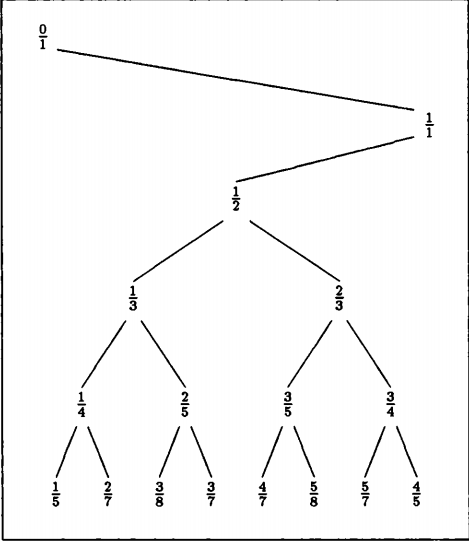
\includegraphics[width=9cm]{picture}
\caption{Дерево Штерна --- Броко}
\end{figure}

\renewcommand{\figurename}{Алгоритм}

В этом дереве каждый элемент, исключая первые два, получает-\linebreak
ся как медиана его двух самых близких возрастающих: самый первый\linebreak
среди расположенных слева (самый большой минорант среди возраста-\linebreak
ющих) и самый левый среди расположенных справа (самый малый ма-\linebreak
жорант среди возрастающих).\\
\textbf{Обозначения:} Во всем упражнении $a, a', a"$ обозначают три положи-\linebreak
тельных рациональных числа, представимых в виде $\frac{p}{q}$, $\frac{p'}{q'}$ и $\frac{p''}{q''}$ в несо-\linebreak
кратимой форме, соответственно.\pagebreak

%259 старинца

\noindent\hspace*{10pt}\textbf{a.} Если две дроби $a$ и $a'$, удовлетворяют соотношению $p'q — pq' = 1$,\linebreak
то доказать, что их медианное число получается в несократимом виде.\linebreak
Вывести отсюда, что в конструкции Штерна — Броко все полученные\linebreak
дроби будут несократимы и что этот процесс приводит к упорядочен-\linebreak
ной последовательности дробей. Доказать, что к тому же каждое ра-\linebreak
циональное число из интервала [0,1] достигается некоторой вершиной\linebreak
дерева. Указание: Доказать, что если $\frac{и}{с}$ находится строго между двумя\linebreak
последовательными дробями построения $\frac{p}{q}$ и $\frac{p'}{q'}$, то $c\geq q+q'.$\\
\hspace*{10pt}\textbf{b.} Ряд Фарея порядка $N$ — это последовательность $\mathcal{F}_N$  рациональ-\linebreak
ных чисел из интервала [0,1], представимых в виде несократимых дро-\linebreak
бей, знаменатели которых не превосходят $N$. Вывести из предыдущей\linebreak
задачи алгоритм, который представляет $\mathcal{F}_N$ для возрастающих значе-\linebreak
ний $N$ (вычисление $\mathcal{F}_N$ основывается на $\mathcal{F}_{N-1}$) .\\
\hspace*{10pt}\textbf{c.} Если $a$ и $a'$ — два последовательных члена $\mathcal{F}_N$, то доказать, что\linebreak
$q + q' > N$.\\
\hspace*{10pt}Использовать свойство, доказанное в пункте \textbf{a}, что если $a, a', a"$ —\linebreak
три последовательных члена ряда Фарея (или дерева Штерна — Броко),
то
\begin{equation*}
\frac{p'}{q'}=\frac{p+q''}{q+q''},\;\; p''q-pq''=\lfloor(q+N)/q'\rfloor \text{\;\;\;и\;\;\;} \begin{cases} p''=\lfloor(q+N)/q' \rfloor p'-p, \\q''=\lfloor(q+N)/q' \rfloor q'-q. \end{cases}
\end{equation*}
Это последнее свойство позволяет дать алгоритм, который из ничего\linebreak
порождает все элементы $\mathcal{F}_N$.\\
\hspace*{10pt}\textbf{d.} Пусть $p$ и $q$ — два взаимно простых целых числа, причем $p < q$.\linebreak
Показать, что получение дроби $\frac{p}{q}$ в процессе Штерна — Броко дает не\linebreak
менее двух пар коэффициентов Безу для $p$ и $q$ и что одна из этих пар —\linebreak
самая малая пара коэффициентов Безу для $p$ и $q$.
\\
\\
\noindent\textbf{36. Вычисление коэффициентов Безу $n$-ки целых чисел}\\\\
\hspace*{10pt} Предполагая, что известна функция Безу для двух целых аргумен-\linebreak
тов, дающая пару коэффициентов Безу в качестве передаваемых пара-\linebreak
метров, написать и реализуйте алгоритм вычисления коэффициентов\linebreak
Безу n-ки целых чисел.
\\
\\
\noindent\textbf{37. Экспериментальная проверка теоремы Дирихле}\\\\
\hspace*{10pt} Написать программу, иллюстрирующую теорему Дирихле: «вероят-\linebreak
ность взаимной простоты двух целых чисел равна $6/\pi^2$».\pagebreak

%260 старинца

\noindent\textbf{38. Произведение рядов и арифметическое произведение}\\\\
\hspace*{10pt} Проверить равенство для двух рядов
\begin{equation*}
\sum_{n\geq1}\frac{f(n)}{n^\alpha}\times \sum_{n\geq1}\frac{g(n)}{n^\alpha}=\sum_{n\geq1}\frac{(f*g)(n)}{n^\alpha},
\end{equation*}
где $f * g$ — арифметическое произведение $f$ и $g$. Что можно отсюда\linebreak
вывести, если $f$ и $g$ взаимно обратные функции (в арифметическом\linebreak
смысле)?
\\
\\
\noindent\textbf{39. Сложность центрированного деления}\\\\
\hspace*{10pt} Изучим в этом упражнении сложность алгоритма Евклида, поро-\linebreak
жденного центрированным делением, т.е. делением $a = bq + r$, где\linebreak
$|r|\leq|b|/2$. Для этого введем последовательность $(G_n )_{n\in N}$, определяе-\linebreak
мую через $G_o = 0, G_1 = 1, G_{n +2} = 2G_{n +1} + G_n$.\\
\hspace*{10pt}\textbf{a.} Вычислить первые члены этой последовательности. Проверить,\linebreak
что $G_n\leq G_{n+1}/2$. Полагая при $n \geq 1$ $a = G_n + G_{n - 1}, b = G_n$, доказать,\linebreak
что $0 < b < a$ и что число делений алгоритма Евклида, вычисляющего\linebreak
НОД$(a,b)$, равно $n$.\\
\hspace*{10pt}\textbf{b.} Пусть $a$ и $b$ — два целых числа, для которых $0 < b < a$. Пред-\linebreak
положим, что алгоритм Евклида, применяемый к $(a,b)$, требует $n$ де-\linebreak
лений. Доказать, что $G_n\leq b$ и $G_n + G_{n - 1} \leq a$. Вывести отсюда, что\linebreak
$n<\log_{1+\sqrt{2}}{(b+1)}2\sqrt{2}.$\\
\noindent\textbf{Указание:} если $r_0, r_1$, . . . , $r_{n}$ и $r_{n+1}= 0$ обозначает последователь-\linebreak 
ность остатков, то показать, что $|r_{i-1}|\geq2|r_i|+|r_{i+1}|$ при $i = 2,3,$ . . . $n.$\linebreak
Кроме того, можно доказать, что
\begin{equation*}
G_n=\frac{(1+\sqrt{2})^n-(1-\sqrt{2})^n}{2\sqrt{2}}
\end{equation*}\\
\hspace*{10pt}\textbf{c.}  Пусть $p$ — число десятичных цифр в записи $b$. Доказать, что\linebreak
$n\leq \alpha p +\beta $, где $\alpha$ и $\beta$ следующие: $\alpha+1/\log_{10}{1+\sqrt{2}}\approx2,612496$ и\linebreak
$\beta = \log_{10}{(2\sqrt{2})}/\log_{10}{(1+\sqrt{2})} \approx 1,17965.$\\
\hspace*{10pt} Вывести отсюда, что число центрированных делений, необходимых\linebreak
для вычисления НОД двух положительных целых чисел, не превосходит\linebreak
утроенного числа цифр наименьшего из этих чисел.
\\
\\
\noindent\textbf{40. Порождения простых чисел с помощью многочленов}\\\\
\hspace*{10pt}\textbf{a.} Доказать, что не существует непостоянного многочлена с це-\linebreak
лыми коэффициентами, который принимает только простые значения.\linebreak
Указание: вычислить $P(n+P(n))$.\pagebreak

%261 старинца

\noindent\hspace*{10pt}Согласно постулату Бертрана, для любого целого $n > 1$ в интервале\linebreak
$]n, 2n[$ существует простое число.\\
\hspace*{10pt}\textbf{b.} Доказать, что если $p_i$ означает $i$-ое простое число, то\\
$p_{n+1}\leq p_1+\cdot\cdot\cdot+p_n$ для $n>1$.\\
\hspace*{10pt}\textbf{c.} Использовать постулат Бертрана для доказательства существо-\linebreak
вания такого вещественного числа $K$, что $n$-ое простое число есть целая\linebreak
часть от $10^{n{^2}} K$ mod $10^n$.
\\
\\
\noindent\textbf{41. Соотношение Безу для многочленов}\\\\
\hspace*{10pt}Пусть $P$ и $Q$ — два постоянных многочлена с коэффициентами в\linebreak
факториальном кольце $A$ с полем частных $K$ . Доказать, что $P$ и $Q$\linebreak
взаимно просты (в $K [X]$) тогда и только тогда, когда найдутся та-\linebreak
кие два многочлена $U$ и $V$ с коэффициентами в $A$, что deg$U$ < deg$Q$,\linebreak
deg$V$ < deg$P$, и элемент $\alpha \in A$, отличный от нуля, что $UP + VQ = \alpha.$
\\
\\
\noindent\textbf{42. Сложность алгоритма Евклида в $K[X]$}\\\\
\hspace*{10pt}Рассмотрим сложность алгоритма Евклида в $K[X]$, где $K$ — нётеро-\linebreak
во поле. Алгоритм, в котором используется обычное деление: $A = BQ +\linebreak
R$ с deg ($R$) < deg ($B$). Обозначим через $\varphi$ отображение в $K[X] \times K[X]$ в $\mathbb{N}$,\linebreak
которое паре многочленов ($A$, $B$) ставит в соответствие число делений,\linebreak
необходимых для получения НОД ($A$, $B$).\\
\hspace*{10pt}\textbf{a.} Доказать, что $\varphi (A,B)\leq 1 + $deg($B$).\\
\hspace*{10pt}\textbf{b.} Доказать, что эта оценка наилучшая возможная: можно указать\linebreak
последовательность $(F_n(X))_{n\geq0}$ для которой: deg($F_n$) = $n$ и\linebreak
$\varphi(F_n , F_{n-1}) = n (= 1 + deg(F_{n-1}))$.
\\
\\
\noindent\textbf{43. Оптимальность алгоритма для $K[X]$ (теорема Лазара)}\\\\
\hspace*{10pt}Цель этого упражнения доказать, что среди всех алгоритмов «$\grave{a}$ $la$\linebreak
Евклид» вычисления НОД в $K[X]$ наилучшим является алгоритм, ис-\linebreak
пользующий обычное евклидово деление многочленов. Обозначим че-\linebreak
рез $\varphi: K[X] \times K[X] \rightarrow \mathbb{N}$ минимальный квазиалгоритм (см. раздел 6.2)\linebreak
в $K[X]$ и через  $\varphi$ сложность алгоритма с использованием обычного\linebreak
деления. Докажем равенство  $\mu=\varphi$.\\
\hspace*{10pt}\textbf{a.} Для $A, A', B$ из $K[X]$ и константы $k$, отличной от 0, проверить\linebreak
следующие соотношения для $\mu$ и $\varphi$:
\begin{equation*}
\mu(A,B)=0\Leftrightarrow B=0,
\end{equation*}
\begin{equation*}
\mu(kA,B)=\mu(A,kB)=\mu(A,B),
\end{equation*}
\begin{equation*}
\mu(A,B)+\mu(A',B)\;\; \text{если}\;\;A\equiv A'\;(\text{mod }B). 
\end{equation*}\pagebreak

%262 старинца

\noindent\hspace*{10pt}\textbf{b.} Пусть $A$, $B$ в $K[X]$. Доказать, используя индукцию по значениям\linebreak
$\mu$, что $\mu(A ,B ) = \varphi(A, B)$. Указание: введите остатки $R$ и $R'$ от обыч-\linebreak
ного и оптимального деления $A$ на $B$. Затем рассмотреть 3 случая:\linebreak
deg($R$) < deg($B$), deg($R$) > deg($B$), deg($R$) = deg($B$).
\\
\\
\noindent\textbf{44. К теореме Лаэара}\\\\
\hspace*{10pt} Рассмотрим последовательность $C_0 = 0,$ $ C_1 = 1$ и $C_{2i} = ЗC_{2i-1} +$\linebreak
$C_{2i-2},$ $C_{2i+1}=2C_{2i}-C_{2i-1}$. Доказать, что алгоритм, использующий\linebreak
\textit{центрированное} деление, примененный к ($C_{n+1}$, $C_n$), требует $n$ деле-\linebreak
ний. Доказать также, что используя «одно на двоих» не центрирован-\linebreak
ное деление, приходим к алгоритму той же сложности (т.е. необходимо\linebreak
$n$ делений, хотя используется $\lfloor\frac{n-1}{2}\rfloor$ нецентрированных делений).
\\
\\
\noindent\textbf{45. (Неэффективное) решето Эратосфена для многочленов}\\\\
\hspace*{10pt}\textbf{a.} Дан список целых чисел от 2 до $n$. Решето Эратосфена позволяет,\linebreak
вычеркивая кратные числа, оставить в нем лишь те, которые являются\linebreak
простыми. Написать алгоритм, реализующий это решето.\\
\hspace*{10pt}\textbf{b.}  Пусть $p$ — целое простое число. Найти в явном виде биективное\linebreak
отображение множества натуральных чисел $\mathbb{N}$ во множество унитарных\linebreak
непостоянных многочленов над $\mathbb{Z}/p\mathbb{Z}$. Если $n\geq 1$, то каким является\linebreak
множество $B_n$ унитарных непостоянных многочленов степени $\leq n$ по\linebreak
модулю $p$?\\
\hspace*{10pt}\textbf{c.} С помощью предыдущего кодирования записать алгоритм «реше-\linebreak
та Эратосфена», который дает список унитарных неприводимых мно-\linebreak
гочленов по модулю $p$ степени $\leq n$. Этот алгоритм является неэффек-\linebreak
тивным по многим причинам. Каким?\\
\hspace*{10pt}\textbf{d.} Написать программу на языке Си, позволяющую найти пере-\linebreak
чень неприводимых многочленов по модулю 2 степени $\leq n$ для доста-\linebreak
точно малого числа $n$ (например, $n\leq 10$).
\\
\\
\noindent\textbf{46. Многочлены $X^n-1$}\\\\
\hspace*{10pt}Пусть $m$ и $n$ — целые неотрицательные числа, $d$ — их НОД.\\
\hspace*{10pt}\textbf{a.} Показать, что $\mathbb{Z}[X](X^d - 1) = \mathbb{Z}[X](X^n - 1) + \mathbb{Z}[X](X^m - 1)$.\linebreak
Вывести отсюда, что в любом кольце $A$ имеем $A(a^d - 1) = A(a^n - 1) +\linebreak
A(a^m - 1)$ для $a \in A$ и что НОД($a^n-1, a^m - 1) = a^d - 1$. В частности,\linebreak
НОД($X^n - 1 ,X^m - 1) =X^d - 1$.\\
\hspace*{10pt}\textbf{b.} Если $f(X )$ и $g(X)$ — два унитарных многочлена с целыми ко-\linebreak
эффициентами, a $h(X)$ — их НОД, $a$ — целое число, то верно ли, что\linebreak
$h(a) =$ НОД$(f(a), g(a))$?\pagebreak

%263 старинца

\noindent\hspace*{10pt}\textbf{c.} Если $m$ > 0, то каков остаток от деления $X^n  - 1$ на $X^m -1$?
\\
\\
\noindent\textbf{47. Неприводимые многочлены над $\mathbb{Z}$}\\\\
\hspace*{10pt} Показать, что многочлены $P_k=X^{2^{k}}+1$ и $Q_n=X^n-2$, неприводимы\linebreak
в $\mathbb{Z}[X]$.
\\
\\
\noindent\textbf{48. Оценка числа неприводимых множителей}\\\\
\hspace*{10pt} Возьмем $A$ — кольцо без делителей нуля.\\
\hspace*{10pt}\textbf{a.} Пусть $A$ — факториальное кольцо. Доказать, что если найдется\linebreak
неприводимый элемент $p$ такой, что показатель $a$ в $p$, $v_p(a)$ равен 1, то\linebreak
полином $X^n$ - $a$ неприводим ($v_p(a)$ есть показатель $p$ в разложении $a$ в\linebreak
произведение неприводимых).\\
\hspace*{10pt}\textbf{b.} Пусть $I$ — простой идеал в кольце $A$ (не обязательно фактори-\linebreak
альном) и пусть $P=a_nX^n+\cdot\cdot\cdot+a_0$ такой, что $a_n\notin I$ и для $i\neq n:a_i\in I$.\linebreak
Показать, что всякий непостоянный делитель $P$ имеет свободный член,\linebreak
содержащийся в $I$.\\
\hspace*{10pt}\textbf{c.} Пусть $A$ — факториально. Доказать, что всякий многочлен, для\linebreak
которого найдется неприводимый элемент $p$ такой, что $p\nmid a_n$ и $p\;|\;a_i$\linebreak
для всех $a_i$ имеет не более $u_p(a_0)$ неприводимых сомножителей.
\\
\\
\noindent\textbf{49. Неприводимый многочлен, приводимый по модулю\\
всякого простого числа}\\\\
\hspace*{10pt}\textbf{a.} Проверить, что многочлен $X^4+1$ приводим по модулю 2.\\
\hspace*{10pt}\textbf{b.} Пусть $p$ — простое число, отличное от 2. Доказать, что число\linebreak
квадратов в группе обратимых элементов $U(\mathbb{Z}/p\mathbb{Z})$ равно числу не-\linebreak
квадратов. Вывести отсюда, что произведение двух не-квадратов есть\linebreak
квадрат.\\
\hspace*{10pt}\textbf{c.} Записав $X^4+1$ в одной из трех форм: $X^4-(-1),\;(X^2+1)-2X^2$ или\linebreak
$(X^2-1)^2-(-2X^2)$, доказать, что многочлен $X^4+1$ приводим по модулю\linebreak
$p$. Дайте примеры для разных значений $p$. Что можно утверждать, если\linebreak
$p \equiv 1$ (mod 4)?\\
\hspace*{10pt}\textbf{d.} Многочлен $X^4+1$ неприводим по модулю 25? А по модулю 15?
\\
\\
\noindent\textbf{50. Нули многочленов с целыми коэффициентами}\\\\
\hspace*{10pt}\textbf{a.} Пусть $P=\sum a_iX^i$ — унитарный многочлен с целыми коэффи-\linebreak
циентами. Доказать непосредственно, что всякий рациональный корень\linebreak
$P$ является в действительности целым и что он делит $a_0$.\pagebreak

%264 старинца

\noindent\hspace*{10pt}\textbf{b.} Пусть $P=\sum_{i\leq n}a_iX^i$ — многочлен, свободный член которого\linebreak
отличен от нуля. Существует ли рациональный корень $p/q$ этого мно-\linebreak
гочлена, где $p/q$ — несократимая дробь, такой, что $p\;|\; a_0$ и $q \;|\; a_n$ .
\\
\\
\noindent\textbf{51. Расширенный критерий Эйзенштейна}\\\\
\hspace*{10pt}\textbf{a.} Пусть  $P=\sum_{i\leq n}a_iX^i$ — многочлен с коэффициентами в факто-\linebreak
риальном кольце. Пусть $p$ — неприводимый элемент в $A$ и $k\leq n$ такое,\linebreak
что  $p^2 \nmid a_0, p \nmid a_k$ и $p \;| \;a_i$ для всех $i < k$. Доказать, что по меньшей мере\linebreak
один из неприводимых делителей $P$ имеет степень, не меньшую $k$.\\
\hspace*{10pt}\textbf{b.} Доказать, что многочлен $P=X^4+3X^3+3X^2-5$ неприводим.\linebreak
При каких значениях а многочлен $Q=5X^4-6X^3-aX^2-4X+2$\linebreak
неприводим? Дайте возможные разложения.
\\
\\
\noindent\textbf{52. Неприводимость циклотомических многочленов}\\\\
\hspace*{10pt} Определим циклотомический многочлен уровня $n$ как $\Phi_n(X)$ =\linebreak
$\prod (X-\xi)$, где произведение распространено на все первообразные корни\linebreak
$n$-й степени из единицы в $\mathbb{C}$. В главе V будет доказано, что коэффици-\linebreak
енты этих многочленов — целые числа. В упражнении этот факт будет\linebreak
использоваться как известный результат.\\
\hspace*{10pt}\textbf{a.} Пусть $\alpha\in \mathbb{C}$ корень $n$-й степени из 1 и $P$ — неприводимый де-\linebreak
литель $X^n -1$, для которого $\alpha$ является корнем. Доказать, что если\linebreak
$p$ — простое число, не делящее $n$, то $P (\alpha^p)=0$. Указание: предположи-\linebreak
те, что $X^n -1=PQ$, и показать, что $P\;|\;Q(X^p)$. Перейдите затем в\linebreak
$\mathbb{Z}/p\mathbb{Z}[X]$.\\
\hspace*{10pt}\textbf{b.} Вывести отсюда, что $\Phi_n$ неприводим.
\\
\\
\noindent\textbf{53. Идеалы в $K[[X]]$}\\\\
\hspace*{10pt} Определить все идеалы в $K[[X]]$, кольце формальных рядов с коэф-\linebreak
фициентами в поле $K$.
\\
\\
\noindent\textbf{54. О факториальных кольцах}\\\\
\hspace*{10pt}\textbf{a.} Пусть $\mathcal{P}$ — система представителей неприводимых элементов\linebreak
факториального кольца $A$ (каждый неприводимый элемент из $A$ ассо-\linebreak
циирован с одним и только одним неприводимым в $\mathcal{P}$). Обозначим через\linebreak
$\mathbb{N}^{(\mathcal{P})}\subset \mathbb{N}^{(\mathcal{P})}$ множество семейств целых чисел $(v_p)_{p\in\mathcal{P}}$, таких, что $v_p= 0$\linebreak
для всех, за исключением конечного числа элементов в $p$. Изучите свой-\linebreak
ства отображения:
\begin{equation*}
\varphi: U(A)\times \mathbb{N}^{(\mathcal{P})}\rightarrow A-\{0\},\;\;\;\varphi(\epsilon,(v_p)_{p\in \mathcal{P}})=\epsilon\prod_{p\in \mathcal{P}}^ {}p^{v_p}.\pagebreak
\end{equation*}

%265 старинца

\noindent Вывести отсюда, что в факториальном кольце любые два элемента име-\linebreak
ют НОД и что множество главных идеалов нётерово по включению.\\
\hspace*{10pt}\textbf{b.}  В факториальном кольце выполняются следующие свойства:
\begin{equation*}
c\;\text{НОД}(a,b)=\text{НОД}(ca, cb), c\;\text{НОК}(a,b)=\text{НОК}(ca, cb)
\end{equation*}
\begin{equation*}
[a\;|\;bc \text{ и НОД}(a,b)=1]\Rightarrow a\;|\;c,\;\;\;[a\;|\;c \text{ и }b\;|\;c \text{ и НОД}(a,b)=1]\Rightarrow ab\;|\;c.
\end{equation*}
\noindent 
Как доказать? Можно ли дать другое доказательство в случае, когда\linebreak
кольцо является КГИ?
\\
\hspace*{10pt}\textbf{c.} Пусть $A$ — кольцо без делителей нуля. Доказать, что $A$ фак-\linebreak
ториально тогда и только тогда, когда некоторые два элемента имеют\linebreak
НОД и множество главных идеалов $A$ является нётеровым. Кроме того,\linebreak
всякий неприводимый элемент является простым и множество главных\linebreak
идеалов нётерово.
\\
\\
\noindent\textbf{55. Условия, при которых факториальное кольцо является\\
кольцом главных идеалов}\\\\
\hspace*{10pt} В пунктах \textbf{a} и \textbf{b} $A$ означает факториальное кольцо.\\
\hspace*{10pt}\textbf{a.} Пусть всякий неприводимый элемент $A$ порождает максималь-\linebreak
ный идеал. Доказать, что $A$ есть КГИ. Указание: доказать, что лю-\linebreak
бой простой идеал главный, потом доказать, что $Ax+Ay=Ad$, если\linebreak
$d=$ НОД($x,y$).
\\
\hspace*{10pt}\textbf{b.} Допустим, что $A$ удовлетворяет соотношению Безу (т. е. если $x$\linebreak
и $y$ взаимно просты, то $1\in Ax+Ay$). Доказать, что $A$ есть КГИ.
\\
\hspace*{10pt}\textbf{c.} Доказать, что конечное кольцо без делителей нуля есть поле.\linebreak
Лучше: если $R$ — алгебра без делителей нуля, конечной размерности\linebreak
над полем $K$, то $R$ — тело ($R$ не предполагается коммутативной). Еще\linebreak
лучше: если $R$ алгебра без делителей нуля, алгебраическая над полем\linebreak
$K$, то $R$ — тело.
\\
\hspace*{10pt}\textbf{d.} Пусть $A$ — подкольцо в $\mathbb{C}$, целое для $\mathbb{Z}$ (например, кольцо целых\linebreak
числового поля). Доказать, что всякий собственный простой идеал $A$,\linebreak
отличный от нуля, максимален. Указание: Если $I$ такой идеал, то дока-\linebreak
зать, что $I \cap\mathbb{Z}$ имеет вид $p\mathbb{Z}$, где $p$ — простое число. Затем рассмотреть\linebreak
$\mathbb{Z}/p\mathbb{Z}$-алгебру $A/I$. Вывести отсюда, что если $A$ факториально, то $A$ -\linebreak
КГИ.
\\
\\
\noindent\textbf{56. Произведение упорядоченных нётеровых множеств}\\\\
\hspace*{10pt} Пусть $(E_i)_{i\in I}$ — семейство упорядоченных множеств. Наделим\linebreak
$\prod_{i\in I} E_i$ структурой упорядоченного произведения, положив $x\leq y$ то-\linebreak
гда и только тогда, когда $x_i\leq y_i$ для всякого $i\in I$. В частности, если\linebreak\pagebreak

%266 старинца

\noindent $E_i=E$ для любого $i$, то $\prod_{i\in I} E_i=E^I$ есть пространство функций из $I$\linebreak
в $E$, наделенное обычным порядком.\\
\hspace*{10pt}\textbf{a.} Доказать, что конечное произведение множеств нётерово тогда\linebreak
и только тогда, когда каждый из множителей нётеров.\\
\hspace*{10pt}\textbf{b.} Рассмотрим подмножество $S \subset E^\mathbb{N}$ состоящее из стабилизирую-\linebreak
щихся последовательностей. Доказать, что в общем случае из нётеро-\linebreak
вости $E$ не следует нётеровость $S$ (а тем более и $E^\mathbb{N}$).
\\
\hspace*{10pt}\textbf{c.} Доказать, что подмножество  $E^\mathbb{N}$, состоящее из возрастающих\linebreak
последовательностей, является нётеровым, если таковым является $E$.
\\
\hspace*{10pt}\textbf{d.} Установите связь между этими результатами и результатами\linebreak
о модулях (нётеровость произведения или частного двух модулей над\linebreak
кольцом многочленов).
\\
\\
\noindent\textbf{57. Конечные (коммутативные) поля}\\\\
\hspace*{10pt} В этом упражнении предполагается доказать несколько вполне клас-\linebreak
сических результатов, касающихся конечных полей. В частности, что\linebreak
для любой степени $q$ простого числа существует одно и только одно\linebreak
(с точностью до изоморфизма) конечное поле из $q$ элементов. Для по-\linebreak
лучения более подробных сведений читатель может обратиться к [111]\linebreak
или [120]. В частности, в [120] можно найти доказательство принадле-\linebreak
жащего Веддербарну результата о том, что всякое конечное тело ком-\linebreak
мутативно.\\
\hspace*{10pt}
Тела, рассматриваемые в этом упражнении, \textbf{заведомо коммута-\linebreak
тивны за исключением пункта (а)}. Бели $A$ — унитарное кольцо,\linebreak
не обязательно коммутативное, то $\mathbb{Z} \ni m\rightarrow m\cdot1\in A$ есть морфизм. Его\linebreak
ядро, следовательно, есть идеал в $\mathbb{Z}$ вида $m\mathbb{Z}$ для единственного $m\geq0$.\linebreak
Упомянутое целое число $m$ есть, следовательно, наименьшее целое число\linebreak
(в смысле отношения порядка, но также и в смысле делимости) такое,\linebreak
что $m\cdot1=0$ или по другому $m\cdot x=0$ для всякого $x\in A$ (такое $m$ \linebreak
называется \textit{характеристикой кольца} $A$).
\\
\hspace*{10pt}\textbf{a.} Доказать, что характеристика кольца без делителей нуля есть\linebreak
или 0, или простое число $p$. В случае поля $K$ доказать, что отображение\linebreak
$m\mapsto m\cdot1$ задает морфизм (инъективный) поля $\mathbb{Q}\rightarrow K$ или $\mathbb{Z}/p\mathbb{Z}\rightarrow K$.\linebreak
Конечное поле имеет характеристику $p > 0$. Если $K\subset K'$ два конечных\linebreak
поля, то доказать, что $|K'|$ есть степень $|K|$ (в частности, если $K$ —\linebreak
конечное поле характеристики $p$, то $|K|$ — степень р).\\
\\
\hspace*{10pt}\textbf{b.} Пусть $q$ — степень простого числа $p$ и $\Omega$ — поле характеристи-\linebreak
ки $p$. Доказать, что если $\Omega$ — поле, состоящее из $q$ элементов, то все\linebreak\pagebreak

%267 старинца

\noindent корни многочлена $X^q-X$ содержатся в $\Omega$. Доказать обратное, рассма-\linebreak
тривая автоморфизм Фробениуса $x \rightarrow x^q$ и показывая, что множество\linebreak
его неподвижных точек $\mathbb{F}_q=\{x\in \Omega\;|\;x^q=x\}$ является \textit{единственным}\linebreak
подполем поля $\Omega$, состоящим из $q$ элементов. Как доказать (неэффек-\linebreak
тивным образом) существование таких полей $\Omega$?

% Замечание
\begin{mynotice}
На этом уровне удобно (но не обязательно) рассма-\linebreak
тривать алгебраически замкнутое поле характеристики $p$. Напо-\linebreak
мним, что алгебраически замкнутым называется поле, в котором\linebreak
всякий непостоянный многочлен имеет корень и, следовательно,\linebreak
разлагается в произведение линейных множителей (можно дока-\linebreak
зать, что всякое поле содержится в алгебраически замкнутом по-\linebreak
ле, см. например, [111]). В этом смысле все поля $\mathbb{F}_q$ “живут” в\linebreak
алгебраически замкнутом поле  $\Omega$.
\end{mynotice}
\hspace*{10pt}\textbf{c.} Пусть $K\subset K'$ — два конечных поля. $|K|=q$, $|K'| = q^n$ . Поинте-\linebreak
ресуемся \textit{промежуточными} полями $H$, т.е. такими, что $K\subset H\subset K'$.\linebreak
Если $d$ — делитель $n$, то доказать, что $\{x\in K'\;|\;x^{q^d}=x\}$ промежу-\linebreak
точное поле с $q^d$ элементами и установите биекцию между делителями\linebreak
$n$ и промежуточными полями. Эта биекция обладает “хорошим” алге-\linebreak
браическим свойством: каким? Если $m$ — какой-либо делитель $n$, то\linebreak
$\{x\in K'\;|\;x^{q^m}=x\}$ — промежуточное поле. Какое у него число эле-\linebreak
ментов? Если $K_1$ и $K_2$ — Два промежуточных поля порядков $q^{d_1}$ и $q^{d_2}$\linebreak
соответственно, то доказать, что $|K_1\cap K_2| = q^d$, где $d =$ НОД($d_1,d_2$).
\\
\hspace*{10pt}\textbf{d.} Пусть $p$ — простое число, $q = p^n$ — степень $p$. Тогда, как из-\linebreak
вестно, существует унитарный неприводимый многочлен $P$ степени\linebreak
$n$. Это позволяет построить конкретное поле $K$ из $q$ элементов, взяв\linebreak
$K=\mathbb{Z}_p[X]/(P)$. Пусть $K'$ — другое “абстрактное” поле из $q$ элемен-\linebreak
тов. Всякий многочлен с коэффициентами в $\mathbb{Z}_p$ может рассматриваться\linebreak
как многочлен с коэффициентами в $K'$. Доказать, что $P$ имеет корень\linebreak
$y$ в $K'$, так как взятие значения в точке $y$ для полиномов из $\mathbb{Z}_p[X]$ зада-\linebreak
%ет гомоморфизм $y:\mathbb{Z}_p[X]\rightarrow K'$, индуцирующий изоморфизм$K$ на $K'$.\linebreak
ет гомоморфизм $y:\mathbb{X}_p[X]\rightarrow K`$, индуцирующий изоморфизм $K$ на $K`$.
Отсюда следует, что любые два конечных поля одинакового порядка\linebreak
изоморфны.
\\
\hspace*{10pt}\textbf{e.} Пусть $K$ — конечное поле из $q$ элементов и $K'$ — расширение $K$\linebreak
степени $n$. Доказать, что отображение $r:x\mapsto x^q$ есть автоморфизм\linebreak
$K'$ порядка $n$, множество неподвижных точек которого совпадает с $K$.\linebreak
Доказать, что всякий автоморфизм $\sigma$ поля $K'$, оставляющий на месте\linebreak
$K$, есть степень $r$.
\pagebreak

%268 старинца

\noindent\textbf{58. У равнение $x^{p^k}=x$ в локальном кольце характеристики $p$}\\\\
\hspace*{10pt} Пусть $A$ унитарное коммутативное кольцо характеристики $p$, т.е.\linebreak
кольцо, в котором $p\cdot1=0$, и $I$ — идеал в $A$. Пример для размышлений\linebreak
— $A = K[T]$, где $K$ — поле характеристики $p$ и $I$ — идеал, порожден-\linebreak
ный неприводимым многочленом. Доказать, что если $q$ — степень $p$, то\linebreak
пространство $S_n$ решений уравнения $X^q= X$ в $A/I^n$ п изоморфно (с по-\linebreak
мощью применения канонического отображения $\pi:A/I^n\rightarrow A/I$) про-\linebreak
странству $S_1$ решений того же уравнения в $A/I$. Этот результат будет\linebreak
применен в главе IV, чтобы определить число неприводимых множите-\linebreak
лей для степени многочлена с коэффициентом в конечном поле.
\\
\hspace*{10pt}\textbf{a.} Без всяких предположений относительно $A$ доказать, что если\linebreak
$x\in A$ обратим по модулю $I$ и по модулю $J$ ($I$ и $J$ — любые идеалы),\linebreak
то $x$ обратим по модулю $IJ$ и, в частности, по модулю $I^n$ для любого\linebreak
целого $n$.
\\
\hspace*{10pt}\textbf{b.} Предположим теперь, что $I$ — максимальный идеал, но не будем\linebreak
налагать ограничений на характеристику кольца $A$ (так что $q$ может\linebreak
быть любым). Доказать, что уравнение $x^q\equiv x\; ($mod $I^n$ ) эквивалентно\linebreak
$x\equiv0\;($mod $I^n$ ) или $x^{q-1}\equiv1\;($mod $I^n$ ).
\\
\hspace*{10pt}\textbf{c.} Обратимся теперь к предложению, сформулированному во вве-\linebreak
дении. Проверить, что $S_n$ и $S_1$ — две подалгебры и что $\pi(S_n)\subset S_1$.\linebreak
Вывести отсюда и из пункта (\textbf{b}), что ограничение $\pi$ на $S_n$ инъектив-\linebreak
но.
\\
\hspace*{10pt}\textbf{d.} Пусть $a$ — элемент в $I$. Рассматривая потенциально бесконечную\linebreak
сумму $a+a^q+a^{q^2}+\cdot\cdot\cdot+ a^{q^i}+\cdot\cdot\cdot$, доказать существование такого $s\in I$,\linebreak
что $s-s^q\equiv a\;($mod $I^n$). Вывести отсюда, что $\pi(S_n)=S_1$.
\\
\hspace*{10pt}\textbf{e.} Можно \textit{обобщить} ситуацию, забыв про идеал $I^n$, и использовать\linebreak
только кольцо $B=A/I^n$. Доказать, что это кольцо содержит един-\linebreak
ственный максимальный идеал $\mathcal{M}$, такой, что $B/\mathcal{M}\simeq A/I$. Утвержда-\linebreak
ется, что это $B$ есть локальное кольцо вычетов $B/\mathcal{M}$ . Как сформу-\linebreak
лировать результаты пунктов (\textbf{b}), (\textbf{c}) в зависимости от $B$ и $B/\mathcal{M}$?\linebreak
Чтобы получить конечный результат, надо наложить ограничения на\linebreak
идеал $\mathcal{M}$. Какое?
\\
\\
\noindent\textbf{59. Эффективное кольцо главных идеалов, не являющееся\\
евклидовым}\\\\
\hspace*{10pt} Кольцо целых чисел в $\mathbb{Q}[\sqrt{-19}]$ есть кольцо $A=\mathbb{Z}[\theta]$, где $\theta=\frac{1+\sqrt{-19}}{2}$.
\\\\
\hspace*{10pt}\textbf{a.} Какому уравнению степени 2 удовлетворяет $\theta$? Возьмите норму\linebreak
$N$ в кольце $A$. Какие элементы обратимы в $A$?\pagebreak

%269 старинца

\noindent\hspace*{10pt}\textbf{b.} Пусть $a\in A$, $b\in A^*$. Доказать возможность эффективного вычи-\linebreak
сления таких $q,r \in A$, что $a = bq + r$ или даже $2a = bq + r$ с $N (r) < N(b)$.
\\
\noindent\hspace*{10pt}\textbf{c.} Доказать явно, что 2 — максимальный элемент в $A$. Если $a =\linebreak
x +\theta y\;\notin2A$, то найти такое $\tilde{a}$, что $a\tilde{a}\equiv1\;($mod $2A$) , $\tilde{a}$ — самое\linebreak
простое, по возможности. Указание: элемент принадлежит $2A$ тогда\linebreak
и только тогда, когда его норма четна (в дальнейшем такой элемент\linebreak
будет называться четным).
\\
\noindent\hspace*{10pt}\textbf{d.} Доказать, что $A$ есть КГИ. Указание: пусть $I$ — ненулевой идеал\linebreak
в $A, b\in I^*$ — элемент с наибольшей нормой. Если $a\in I$, то псевдоде-\linebreak
ление $a$ на $b$ показывает, что $2a \in(b)$. Использовать теперь максималь-\linebreak
ность двойки...
\\
\noindent\hspace*{10pt}\textbf{e.} Написать алгоритм, который для данных $a,b\in A$ находит $u$ и $v$\linebreak
такие, что $ua+vb=$ НОД ($a,b$). Почему не для всех, а для данных $a$ и $b$?\\
\hspace*{10pt}В этом случае доказать, что псевдоделение из вопроса ($\textbf{b}$) позволяет\linebreak
выразить в явном виде $u,v,r\in A,\;\alpha\in\mathbb{N}$, такие, что $r$ есть НОД для $a$\linebreak
и $b$, удовлетворяющий соотношению $2^\alpha r = ua + vb$.\\
\hspace*{10pt} Если $\alpha\geq1$, выразить $2^{\alpha-1}r$ как линейную комбинацию от $2^\alpha r$ и $a$...\\
\hspace*{10pt} Записать алгоритм вычисления коэффициентов Безу в кольце $A$.
\pagebreak
%\end{document}
